	\documentclass[a4paper,12pt,twoside]{article}



\title{Assignment 1b}

\author{Tung X. Nguyen}
\date{\today}

\setcounter{tocdepth}{3}


\usepackage{tikz,pgfplots}

\pgfplotsset{compat=1.10}
\usepgfplotslibrary{fillbetween}
\usepackage{apacite}
\usepackage{bm}
\usepackage{url}
\usepackage{amsmath}
\usepackage{indentfirst}
\usepackage{amssymb}
\usepackage[showframe=false]{geometry}
\usepackage{booktabs}
\usepackage{amsmath}
\usepackage{tabularx}
\usepackage{systeme}

\usepackage{graphicx}
\graphicspath{ {./img/} }

\usepackage[english]{babel}
\usepackage[utf8]{inputenc}
\usepackage{fancyhdr}
\setlength{\headheight}{15.2pt} 
 
\pagestyle{fancy}
\fancyhf{}
\fancyhead[LE,RO]{Tung X. Nguyen}
\fancyhead[RE,LO]{MAT9004: Assignment 1}
\fancyfoot[LE,RO]{\thepage}
\fancyfoot[CE,CO]{\leftmark}

\renewcommand{\headrulewidth}{2pt}
\renewcommand{\footrulewidth}{1pt}
\numberwithin{equation}{section}

\begin{document}
\maketitle
\thispagestyle{empty}

\tableofcontents
\listoffigures
\thispagestyle{empty}


\oddsidemargin = 22pt
\evensidemargin = 22pt
\marginparsep = 10pt
\marginparwidth = 35pt


\section{Introduction}
In most types of sports, physicality is an important indicator of players for their potential to success. This is especially true for basketball, which is a very physical game. Before 1990, basketball players were mostly tall, sometimes skinny men. As time goes by, we see more players with more body mass. This undeniable trend is a proof showing that physique in NBA is gaining more importance.

Inspired by this observation and by my interest in the game, I decided to pick "The importance of physique in NBA" as the topic for this report. In this report, I attemp to answer several key questions:
\begin{itemize}
\item What is the most common physique type in the NBA (from 2000 to 2020) by height and weight?
\item How the distribution of height and weight changes?
\item How physique can affect the draft number of a player?
\item Is there any differences in the physique of non-US players to US players?
\item How physique and Player Efficiency Rating correlated?
\end{itemize}

For the second question, I split the data into 2 groups for comparison: drafted before 2002 and drafted after 2002. For the third question, I use all draft data from 2000 to 2019 to answer. For the final question related to PER, I only use the PER data from two season 2005-2006 and 2018-2019 for comparison.



\section{Data Wrangling}
The subsection \textbf{Data sources} belows shows the description of my sources. All of them are tabular, html data that can be scraped with the help of libraries including Selenium, BeautifulSoup, pandas and csv.
\subsection{Data sources}
\subsubsection{NBA players regular season stats from Official NBA Statistics and Advanced Analytics}Link: \textit{stats.nba.com/players/bio/} 

This website contain the information about players' full name, their age, their draft, height and weight. There is also the information about their draft (including draft year, draft round, draft number) and key perfomance measurement and the team they are playing for, and these information usually changes season after season. The number of players varies each season, but the maximum is 450 (15 players a team multiplied by 30 teams).


\subsubsection{Player Efficiency Rating (PER)} 
Link \textit{insider.espn.com/nba/hollinger/statistics}.

This is a scale developed by John Hollinger, former Vice President of Basketball Operations for the Memphis Grizzlies (an NBA team). This all-in-one formula attempts to calculate a player's contribution per playing minute, taking in consideration key performance items such as field goals, assists, steals, blocks, rebounds, free-throw, three-pointers \cite{wiper}. PER is not the perfect scale to measure a player defensively (as good defensive players are not necessarily excellent blockers or stealers), but it is still one of the most popular tools available to do evaluate players. Figure 1 is a reference table for PER, provided by Hollinger himself.

\begin{figure}[h]
\caption{PER reference guide}
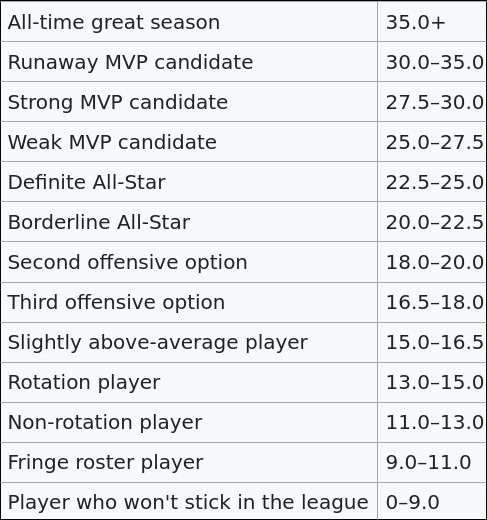
\includegraphics[scale=0.3]{hop.jpg}
\centering
\end{figure}

The PER dataset I used for this assignment is for regular seasons only. Available data includes: the number of games played, minutes per game, true shooting percentage, assist ratio, turnover ratio, usage rate, offensive/defensive rebound rate, PER, value aded, and estimated wins added. Explanation and formula for each of these columns can be found in the end of the data table on the website.


\subsection{Data Cleaning and Transformation}
After the data is saved to csv files, I proceed to transform them into the format I wanted. 

For the NBA players regular season data, I retained only the columns that contain data about physique and draft. Next, I perform union on datasets across seasons from 2000-2001 to 2019-2020 to finally get the data of total 1965 players playing in the NBA from 2000 to 2020. I then remove 57 entries that contains null in physique information. The \textbf{Height} column is originally in feet-inch format, so I used regex to extract tokens and transform this column in to a new column named \textbf{Height\_cm}. \textbf{Weight} is in pound unit.  The result is a dataframe like in Figure 2. The dataframe is sorted according to the \textbf{Draft Year} and \textbf{Draft Round} columns. It can be seen that there are many players who were undrafted, but I decided to keep all these entries (there are 562 undrafted players).

\begin{figure}[h]
\caption{NBA players from 2000 to 2020}
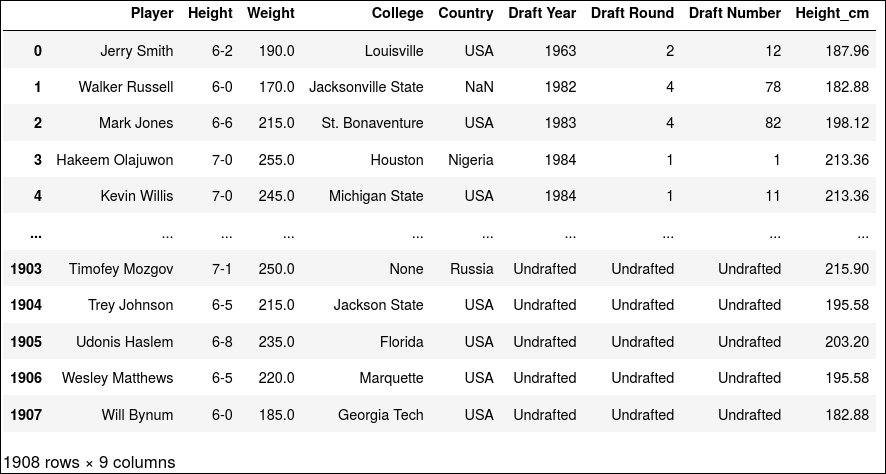
\includegraphics[scale=0.34]{nba_ap.jpg}
\centering
\end{figure}


In the similar manner, I retrieve the PER data for each regular season. I then join (using Python) these data with the physique data above.
\section{Data Checking}

There are some missing in my dataset. Firstly, there are Guy Rucker and Xavier Silas, whose draft number is leave empty in the original dataset. After looking for their information online, I change their draft number to Undrafted.

Next, after merging the PER data with the physique data, I found out that there are some players who were not recorded in the physique data but actually played at the momment. So, I looked up online for their height and weight information to manually fill in the data, using Python.

\section{Data Exploration}
In this section, I use Rstudio to draw plots and explore data.
\subsection{The distribution of Height and Weight}
The distribution of \textbf{Height} for all players from 2000 to 2020 is shown in Figure 3. This distribution is skewed to the right, and the most popular height range is from about 195 to 210 centimeters. 

\begin{figure}[h!]
\caption{Density plot of Height (in cm)}
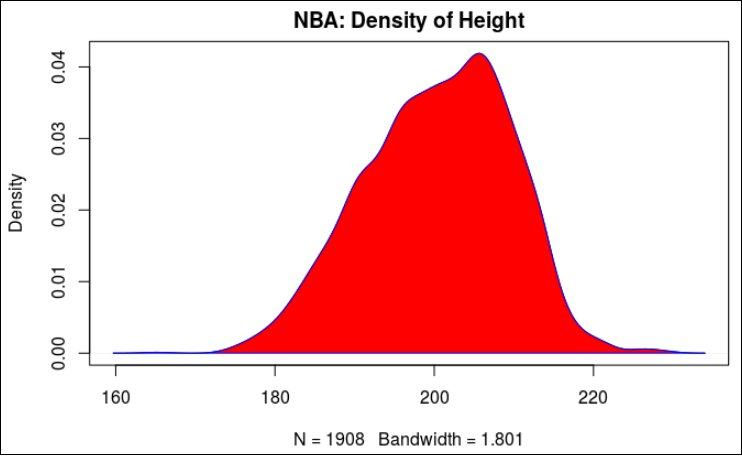
\includegraphics[scale=0.3]{dsoh.jpg}
\centering
\end{figure}

\begin{figure}[h]
\caption{Density plot of Height before vs after 2002}
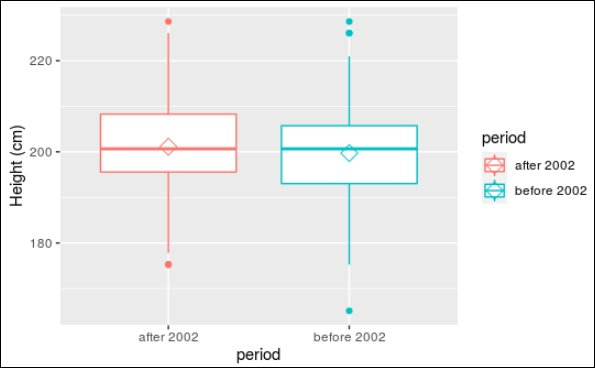
\includegraphics[scale=0.32]{hebf02.jpg}
\centering
\end{figure}

As time goes by, I expect to see the younger generation dominate the older in height. I used the draft year 2002 to split players into 2 groups (each includes roughly 900 players) to compare their height distribution. The result boxplot shown in Figure 4 seems to confirm my speculation. The height mean of the younger group (201.1cm) is higher than that of the older (199.7cm), and the same can be said for the median. Overall, it can said that the height distribution of the younger group is more elevated than that of the older group, which implies that players drafted after 2002 are generally taller than their older counterpart.

\begin{figure}[h]
\caption{Distribution of Weight (in pounds)}
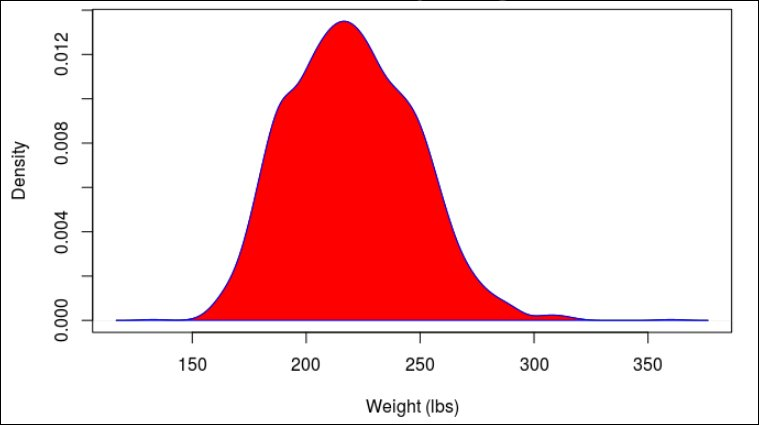
\includegraphics[scale=0.3]{dsow.jpg}
\centering
\end{figure}

\begin{figure}[h]
\caption{Density plot of Weight before vs after 2002}
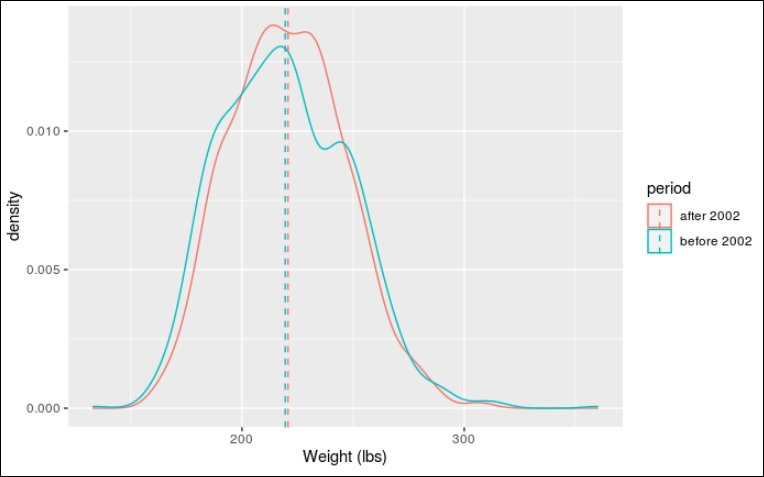
\includegraphics[scale=0.32]{webf02.jpg}
\centering
\end{figure}
I address the same question for \textbf{Weight}, and the result is shown in Figure 5 and Figure 6. The most popular weight range is about 200-230 pounds, and the mean weight for two group are roughly similar. However, the distribution of weight for the younger group are more tightened to the middle, implying a higher percentage of the heavier players, compared to the players drafted before 2002. I use a density plot because the difference is not as recognizable in boxplot.


To conclude this section, I plotted to see how \textbf{Height} and \textbf{weight} are correlated, using a scatter plot in Figure 8. An apparent upward trend is seen in the relationship between \textbf{Height} and \textbf{Weight}. This chart also exposes the outliers in my dataset. There are players who are very heavy for their frame, namely Zion Williamson, Oliver Miller, Shaquille O'Neal, and Sim Bhullar. This can pose huge stress on their knees and ankles, leading to injuries. There are also players who are too skinny, such as Corey Brewer, Shaun Livingston, Zhou Qui and Kristaps Porzingis.

\begin{figure}[h]
\caption{Height and Weight}
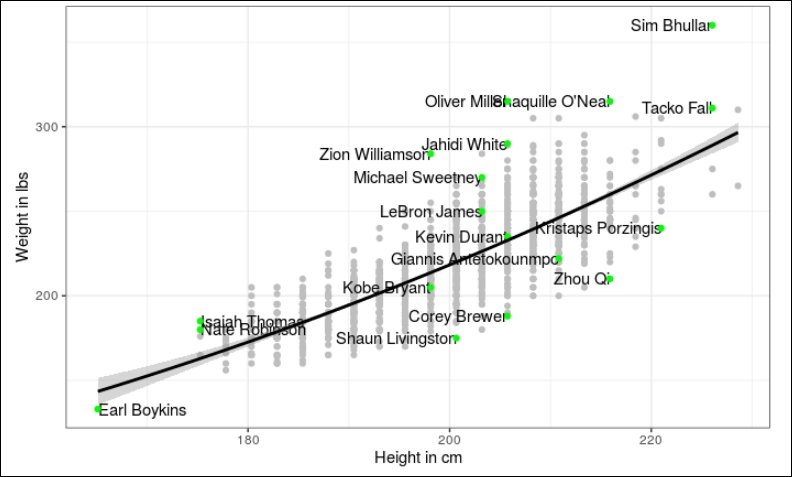
\includegraphics[scale=0.35]{hvw.jpg}
\centering
\end{figure}



\subsection{Draft Number and Height, Weight}

I attempt to find a relationship between \textbf{Draft Number} and \textbf{Height}. but there are no significant pattern found (see Figure 8 belows). The same can be said for the relationship between Weight and Height.s
\begin{figure}[h]
\caption{Draft Number vs Height, Weight}
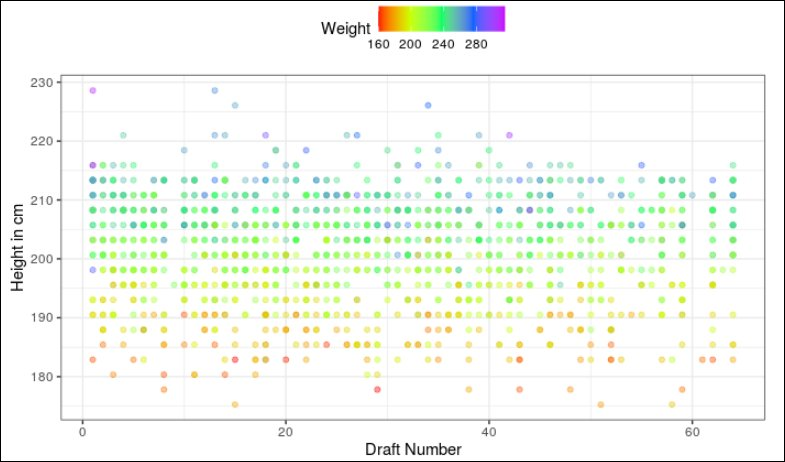
\includegraphics[scale=0.3]{hvdrf.jpg}
\centering
\end{figure}

\subsection{Nationality and Physique}
In 1908 entries in my dataset, there are only 377 foreign players (players who are not from the US). My theory is that foreign players must be physically dominant in order to be noticed by the NBA scouts. 

\begin{figure}[h]
\caption{Height of US vs non-US players}
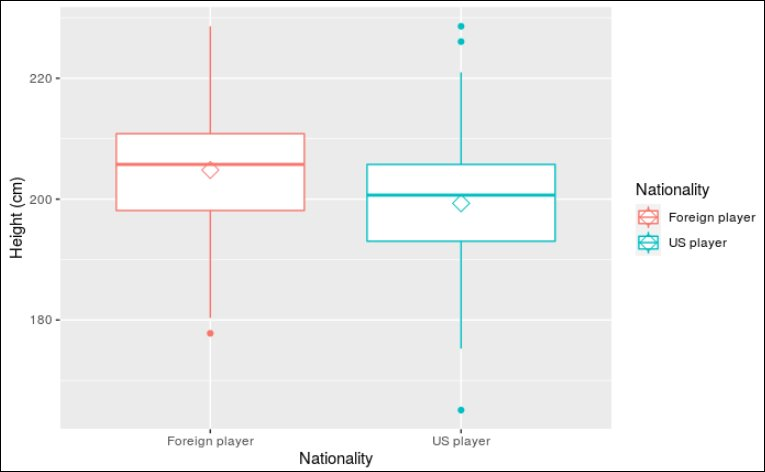
\includegraphics[scale=0.33]{fush.jpg}
\centering
\end{figure}

\begin{figure}[h]
\caption{Weight of US vs non-US players}
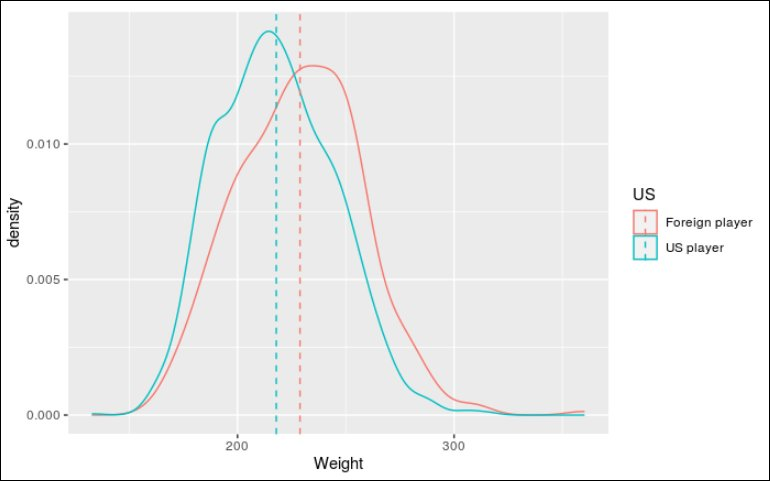
\includegraphics[scale=0.33]{fusw.jpg}
\centering
\end{figure}

It is convincing from the density distribution plots in Figure 9 and 10 that non-US players are more dominant in height and weight: their distribution are more elevated than that of the US counterpart, and comparisons for mean height and weight also agree with my speculation. For example, according to figure 9, 50\% of the foreign group is taller than 75\% of the US group.

\subsection{Physique and PER}
In this section, I will use the PER data for the
 regular season 2018-2019 and 2005-2006 for comparison. I hope to see some differences between two seasons as the game is supposedly modernized now.
 
\begin{figure}[h]
\caption{Height vs PER regular season 2018-2019}
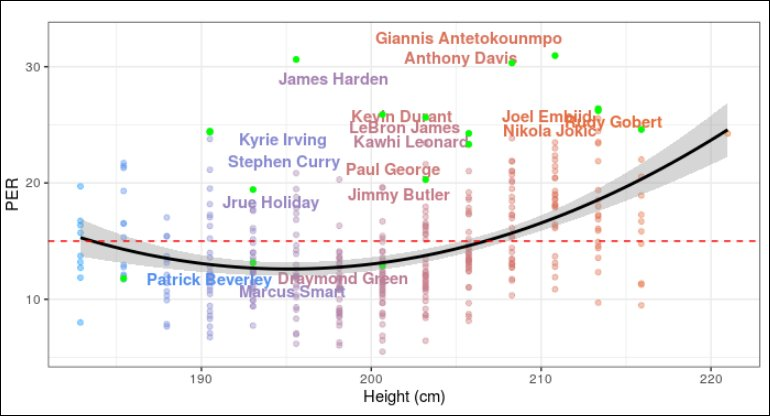
\includegraphics[scale=0.4]{hvsper06.jpg}
\centering
\end{figure}
\begin{figure}[h]
\caption{Height vs PER regular season 2005-2006}
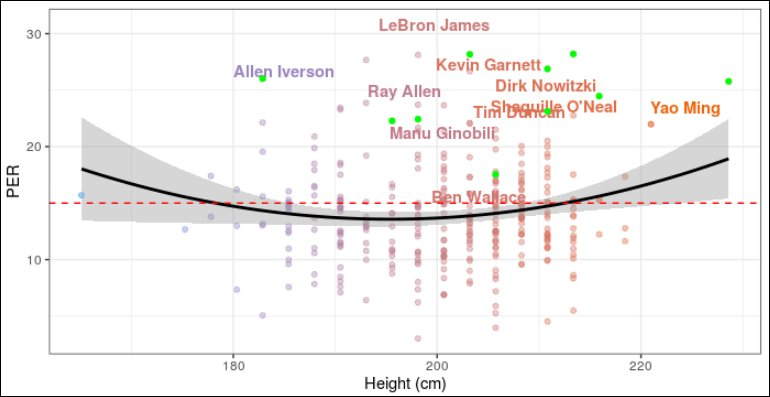
\includegraphics[scale=0.4]{hvsper.jpg}
\centering
\end{figure}

 
The result is shown in Figure 11 and 12. The color of the dots are simply based on \textbf{Height} for easier examination. Both charts reveals an interesting trend that bigger does not always mean better: it seems to be the opposite for players with height below 195cm. As the convex smoothing line implies, taller players (taller than 2m) seems to score higher PER. The trend is more recognizable in regular season 2018-2019, compared to the older time. The elite group also includes players shorter than 2m, such as Allen Iverson (season 2005-2006), Stephen Curry, James Harden, and Kyrie Irving (season 2018-2019), whose skills are exceptional. But, in general, this group is dominated by big, tall, and strong forwards or centers (as the dominance of hot-colored dots implies).

Some of the most defensively successful players are underated by PER, such as Ben Wallace (best defensive player season 2005-2006), Patrick Beverley, Draymond Green, and Marcus Smart (season 2018-2019). The rating for Draymond Green is about 10 only, yet this is one of the best defensive players in the league in recent years.

\section{Conclusion}
In the end, it seems that heavier and taller players are becoming more dominant in the NBA, not only in quantity but also in quality: the highest achievers are usually the strongest players (power forwards or centers). Next, foreign ballers tend to be heavier and taller than US players. Finally, there is no significant proof that draft number is affected by height or weight.

\section{Reflection} 
After this assignment, I became more efficient at scraping and cleaning data using Python. I also got to practice drawing plots using ggplot in Rstudio. I believe that the visualization aspect of my assignment is not too distracting but informative and coherent. 

In subsection \textbf{4.4 Physique and PER}, I did not draw the similar plots for weight because the trend for weight and PER is not as clear as that of height and weight and the report is already too long. And, in order to illustrate the distribution, I had to pick between density plot and boxplot. It seems that sometimes the difference is exposed more in density plot (see Figure 6).

Overall, I am satisfied with the result, but I am open to criticism as there are always rooms for improvement.



 
\bibliographystyle{apacite}
\bibliography{nbabib}


\end{document}
